\chapter{Testování statistických hypotéz}

\section{Základní strategie TSH}
Cílem testování statistických hypotéz je rozhodnout, zda jsme na~základě nějakého experimentu schopni ověřit platnost určitého vysloveného tvrzení (hypotézy) na~úrovni celé populace, případně parametru $\t$ s~touto populací spojeného. Můžeme tak například posoudit, jestli výsledky maturitních testů z~matematiky závisí na~pohlaví a~na~místě narození studentů.
Experiment provádíme na~jednotlivých jedincích,  přičemž často máme k~dispozici tzv. pokusnou a~kontrolní skupinu. Příkladem toho může být například dvojitě zaslepený experiment (\textit{double-blind experiment}), pomocí něhož zkoumáme účinky daného léku. Zde máme dvě skupiny pacientů - první skupině podáváme lék, který chceme otestovat, a~té druhé placebo, případně jiný medikament. Zároveň ale ani pacienti, ani lékaři, neví, které skupině jaký typ léku aplikujeme. Výsledky se~pak zpracují právě užitím testování statistických hypotéz.

Mějme nějaký objekt/subjekt O~a~jeho stav $S\in\mathscr{S}=\mathscr{S}_0+\mathscr{S}_1$ (disjunktní sjednocení $\mathscr{S}_0\cup\mathscr{S}_1$). Testujeme hypotézu
$H_0:\text{ O~je ve~stavu z~}\mathscr{S}_0$ oproti~$H_1:\text{O je ve~stavu z~}\mathscr{S}_1$. Máme-li náhodnou veličinu $X\sim f\in\mathcal{F}$ spojenou se~stavy objektu O~způsobem, že $\mathscr{S}\leftrightarrow\mathcal{F}$ jsou ve~vzájemně jednoznačném vztahu, potom úlohu reformulujeme na
	$$ \hypothesiswide{X\sim f\in\mathcal{F}_0\subset \mathcal{F}}{X\sim f\in \mathcal{F}_1=\mathcal{F}\dotminus\mathcal{F}_0}.$$
	Při případné parametrizaci modelu musíme dbát na~identifikovatelnost rodiny $\mathcal{F}$


\begin{define}
	Mějme populaci $\Omega$ a~na~ní vlastnost $X\sim\FF$, kde \mbox{$\FF\in\mathcal{F}$}. Označme $\t=\t(\FF)$ parametr modelu, který nás zajímá, kde $\t\in\Theta\subset\R^k$. Označme $H_0:\t\in\Theta_0$ jako \textbf{základní nulovou hypotézu} (\textit{null hypothesis}) a~ $H_1:\t\in\Theta_1$, kde \mbox{$\Theta_1=\Theta\setminus\Theta_0$}, jako \textbf{alternativní hypotézu}. 
\end{define}

Nulová hypotéza $H_0$ může označovat "původní stav", tedy že zkoumaná věc se~nezměnila, nebo že je lepší, než nějaký alternativní stav z~hypotézy $H_1$. Ta naproti~tomu  většinou doplňkově vyvrací platnost nulové hypotézy $H_0$, např. že nový lék funguje lépe než starý, nebo že alternativní rozdělení odpovídá naměřeným datům více, než distribuce deklarovaná v~$H_0$. O~zamítnutí $H_0$, resp. přijetí, rozhodujeme na~základě dostupného náhodného výběru $\X=(X_j)_{j=1}^n$ pořízeného v~rámci  zvoleného experimentu.

\begin{example}
	Hypotézou $H_0$ může být například to, že náhodný výběr pochází z~normálního rozdělení, nebo že 2 náhodné výběry pochází ze~stejného rozdělení, případně že mají alespoň stejnou střední hodnotu nebo rozptyl.
	Máme-li dvě výrobní metody a~k~nim příslušné náhodné výběry $X_1,...,X_n\sim\n{\mu_1,\sigma_1^2}$ a~$Y_1,...,Y_m\sim\NN(\mu_2,\sigma_2^2)$, můžeme zkoumat například to, jestli platí $H_0:\mu_1=\mu_2$ (výrobní metody jsou ve~své střední hodnotě stejné), versus $H_1:\mu_1<\mu_2$ (nová metoda č.1 ($X_j$) je lepší, než původní metoda č.2 ($Y_j$)).
\end{example}
\begin{define}
	Definujeme $\rhn$ jako jev představující \textbf{zamítnutí} $H_0$ (\textit{rejection}) a~$\rhno$ jako \textbf{přijetí} $H_0$ (\textit{acception}). Pak \textbf{kritickou funkci testu} definujeme jako pravděpodobnost, že zamítneme $H_0$ na~základě naměřených dat $\textbf{x}$, tzn. $$\crossedphi(\textbf{x}):=\PP(\rhn|\X=\textbf{x})\in[0,1],\quad\text{pro~}\forall\textbf{x}\in\mathcal{X},$$
	kde $\mathcal{X}$ je tzv. \textbf{výběrový prostor}, $\mathcal{X}=\{ \textbf{x}\in\R^n:\exists\omega\in\Omega,~\X(\omega)=\textbf{x} \}$. Dále definujeme pro~test $\hypothesis{\t\in\Theta_0}{\t\in\Theta_1},~\Theta=\Theta_0+\Theta_1$, funkci
	\[\begin{split}
	\beta_\crossedphi(\t)&:=\E_\t[\crossedphi(\X)]=\E_\t[\PP(\rhn|\X=\textbf{x})]=\begin{array}{|l|}
	\PP(A)=\int\limits_{A}1\d \PP=\int\limits_{\Omega}\Identita{A}\d\PP=\E[\Identita{A}]\\ A=\{\rhn|\X=\textbf{x}\} 
	\end{array}=\\&=\E_\t\big[\E[\Identita{\rhn}|\X=\textbf{x}]\big]\equal{\E[\E[X|Y]]=\E X}\E_\t[\Identita{\rhn}]=\PP_\t(\rhn),\quad\text{pro } \forall\t\in\Theta . 
	\end{split}\]
	Funkce $\silofunkce{1}$, tedy zúžení $\beta_\crossedphi$ z~$\Theta$ na~obor $\Theta_1$, se~nazývá \textbf{silofunkce testu} $\crossedphi$.
\end{define}
~\\
Pokud testujeme hypotézu $H_0$ oproti~$H_1$, mohou nastat 4 navzájem se~vylučující situace:\begin{center}
	\begin{tabular}{|l|c|c|}
		\hline 
		& \textbf{Zamítáme $H_0$} & \textbf{Nezamítáme $H_0$} \\ 
		\hline 
		\textbf{$H_0$ platí} & Nastává chyba I. druhu  & Správný výsledek \\ 
		\hline 
		\textbf{$H_0$ neplatí} & Správný výsledek & Nastává chyba II. druhu\\ 
		\hline 
	\end{tabular} 
\end{center}
Chybu I. druhu považujeme za~kritickou (tu horší) chybu. Pravděpodobnost chyby I. druhu vyjadřuje právě funkce $\silofunkce{0}$, což je zúžení $\beta_\crossedphi$ z~$\Theta$ na~obor $\Theta_0$. Právě tuto pravděpodobnost budeme chtít mít pod~kontrolou, tzn. pro~vhodně malé zvolené číslo $\alpha\in(0,1)$ požadujeme, aby celé zúžení $\silofunkce{0}$ bylo stejnoměrně pod~zadanou hranicí $\alpha$. 
Číslo $\alpha$ nazýváme \textbf{hladina významnosti} testu $H_0$ versus $H_1$ a~požadujeme tedy, aby $\sup\limits_{\t\in\Theta_0}\beta_\crossedphi(\t)\leq \alpha.$


Pravděpodobnost chyby II. druhu vyjadřuje funkce $1-\silofunkce{1}$ a~budeme se~ji snažit minimalizovat za~vazební podmínky $\silofunkce{0}\leq \alpha$ na~chybu I. druhu.

\begin{figure}[h]
	\centering
	\begin{tikzpicture}
	\node[inner sep=0pt] (pic) at (0,0)
	{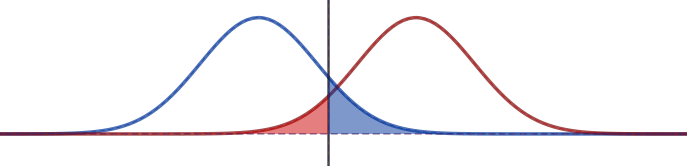
\includegraphics[width=10cm]{Images/hypothesis}};
	\draw [color=blue!20!black](-6.55,1.0) node[anchor=north west] {Alternativní hypotéza $H_1$};
	\draw [color=red!40!black](2.05,1.0) node[anchor=north west] {Nulová hypotéza $H_0$};
	\draw [color=black](-0.65,-0.35) node[anchor=north west] {$\alpha$};
	\draw [color=black](-2.6,1.75) node[anchor=north west] {Volená hranice pro~rozhodnutí mezi~$H_0$ a~$H_1$};
	\draw [color=black](-0.25,-0.25) node[anchor=north west] {$\beta$};
	\draw [color=black](-3.5,-1) node[anchor=north west] {Zamítáme $H_0$};
	\draw [color=black](1,-1) node[anchor=north west] {Nezamítáme $H_0$};
	\end{tikzpicture}
	\caption{Porovnání hypotéz pro~případ jednoduché $H_0$ (jeden stav) oproti~jednoduché $H_1$ (druhý alternativní stav).}
	\label{fig:grafik}
\end{figure}

Shrňme strategii testování $\hypothesis{\t\in\Theta_0}{\t\in\Theta_1}$ v~následující sekci.
\section{UMP testy pro~parametr $\t=\t(\FF)$}
\begin{define}[UMP strategie testování $H_0$ vs. $H_1$] Hledáme takovou optimální kritickou funkci testu $\Phiast$, aby při~zvolené hladině významnosti $\alpha\in(0,1)$ byla pravděpodobnost chyby II. druhu minimální, tzn. aby pro~$\forall\t\in\Theta_1$ bylo $\beta_{\Phiast}(\t)$ stejnoměrně na~$\Theta_1$ \textbf{maximální silou testu}, za~podmínky, že pravděpodobnost chyby I. druhu bude stále (stejnoměrně na~$\Theta_0$) pod~hranicí $\alpha$, tzn. $$\forall\t\in\Theta_0,~\beta_{\Phiast}(\t)\leq\alpha.$$
	Číslo $\sup\limits_{\t\in\Theta_0}\beta_{\Phiast}(\t)$ se~nazývá \textbf{hladina testu} (\textit{size of test $\Phiast$}) a~v~praxi může být ostře pod~nastavenou hranicí \textbf{hladiny významnosti} testu $\alpha$ (\textit{significance level $\alpha$}). 
	
	Konkrétní hodnotu $\beta_{\Phiast}(\t)$ pro~$\t\in\Theta_1$ nazýváme \textbf{síla testu} $\Phiast$ pro~dané $\t\in\Theta_1$, celé zúžení $\silofunkceast{1}$ pak nazýváme \textbf{silofunkce} testu $\Phiast$.
	
	Pokud takový test $\Phiast$ splňující uvedené podmínky existuje, nazýváme ho stejnoměrně nejsilnějším testem $H_0$ oproti~$H_1$, ozn. \textbf{UMP test} (\textit{uniformly most powerful test}). Situaci UMP ilustruje obrázek \ref{fig:UMP}.

\end{define}
	\begin{figure}[h]
	\centering
	\begin{tikzpicture}[scale=1.4]
	\node[inner sep=0pt] (pic) at (0,0)
	{
\includegraphics[width=6.0cm]{Images/test}};
	\draw [color=black](0.75,0.80) node[anchor=north west] {$\beta_\crossedphi(\t)$};
	\draw [color=black](-2.1,-0.85) node[anchor=north west] {$0$};
	\draw [color=black](-1.2,-0.9) node[anchor=north west] {$\Theta_0$};
	\draw [color=black](0.7,-0.9) node[anchor=north west] {$\Theta_1$};
	\draw [color=black](2.15,-0.62) node[anchor=north west] {$\t$};
	\draw [color=black](0.1,-0.1) node[anchor=north west] {$\sup\limits_{\t\in\Theta_0}\beta_\crossedphi$};
	\draw [color=black](-2.0,1.55) node[anchor=north west] {$\beta_\crossedphi$};
	\draw [color=black](-2.1,0.95) node[anchor=north west] {$1$};
	\draw [color=black](-2.1,0.2) node[anchor=north west] {$\alpha$};
	\end{tikzpicture}
	\caption{UMP model testování $\hypothesis{\t\in\Theta_0}{\t\in\Theta_1}$ na~hladině $\alpha$.}
	\label{fig:UMP}
\end{figure}
\begin{remark} Ještě lepší strategií by bylo hledat test $\crossedphi$, který minimalizuje stejnoměrně oba druhy chyb I. a~II. najednou. To však obecně nelze splnit, protože bohužel platí, že pokud se~snažíme snížit pravděpodobnost chyby jednoho druhu, pak pravděpodobnost druhé chyby roste. Tedy chyby I. a~II. druhu jsou komplementární, a~proto musíme volit určitou formu kompromisu (viz. definice UMP testu $\Phiast$). 
\end{remark}
\begin{define}	Pokud $\Theta_0$ je jednoprvková (1 stav), pak $H_0$ nazveme \textbf{jednoduchá} hypotéza (\textit{simple}), v~opačném případě je $H_0$ \textbf{složená} hypotéza (\textit{composite}). Totéž platí pro~$\Theta_1$ a~$H_1$ alternativu.
\end{define}
UMP je tedy test, který má nejvyšší statistickou sílu $\beta$ na~celém $\Theta_1$ $(H_1)$ mezi~všemi možnými testy pod~zadanou hranicí $\alpha$ pro~chybu I. druhu na~$\Theta_0$ $(H_0)$. Je taky dobré si uvědomit, že $\beta$ je pravděpodobnost, že nenastává chyba II. druhu. Takovýto optimální test nutně nemusí existovat. Pokud však existuje, je možné ho pro~speciální případ jednoduché $H_0$ a~jednoduché $H_1$ nalézt pomocí Neyman-Pearsonova lemmatu, které bude uvedeno dále v~sekci \ref{NPL}. 

\begin{define}
	Pokud uvažujeme kritickou funkci ve~tvaru $$\crossedphi(\textbf{x})=\begin{cases}
	1 & \textbf{x}\in W\subset\R^n, \\ 0 & \text{jinak},
	\end{cases}$$ pak $W$ nazveme \textbf{kritický obor testu} (\textit{critical region}). Je to tedy obor naměřených hodnot, při~kterém zamítáme $H_0$. Tomuto tvaru testu se~říká \textbf{neznáhodněný test} a~o~přijetí $H_0$ rozhodujeme následovně: \[
	\begin{split}
	\text{nastává jev }\{\X\in W\} ~&\Rightarrow~\text{zamítáme }H_0, \\ \text{nastává opačný jev }\{\X\notin W\} ~&\Rightarrow~\text{nezamítáme }H_0. 
	\end{split}
	\]\end{define} 
Kritický obor $W$ musí opět splňovat podmínku omezenosti pravděpodobnosti chyby I. druhu ve~tvaru $$ \PP_\t\br{(X_1,...,X_n)\in W}\leq \alpha,~\forall\theta\in\Theta_0, $$ pro~zadanou hladinu významnosti testu $\alpha\in(0,1)$. Příležitostně budeme pro~kritický obor proto užívat označení $W_\alpha$.

Pro stejnoměrně optimální UMP test $\Phiast$ pak odpovídající kritickou oblast značíme $W^\ast$ a~nazýváme ji \textbf{UMP kritickou oblastí testu} (\textit{UMP critical region - UMPCR}).
Pokud tedy $ (x_1,...,x_n)\in W^\ast$, pak zamítneme $H_0$. Opět příležitostně označíme $\txt{UMP}_\alpha,~\Phiast_\alpha$, nebo $W_\alpha^\ast$.

\section{Neyman-Pearsonovo lemma (N-PL)}\label{NPL}
Nyní už přichází na~řadu \textbf{Neyman-Pearsonovo lemma}, které nám umožní najít nejlepší možný test $\Phiast$ pro~případ jednoduché hypotézy $H_0$ (1 stav) oproti~jednoduché alternativě $H_1$ (také pouze 1 stav).
\begin{theorem}[Neyman-Pearsonovo lemma]
	Mějme dvě hypotézy
	\mbox{$ \hypothesis{\t=\t_0}{\t=\t_1}$} a~číslo $\alpha\in(0,1)$ jako hladinu významnosti testu. Označme nyní hustotu pravděpodobnosti \mbox{$f_0:=f(\textbf{x},\t_0)$} a~ $f_1:=f(\textbf{x},\t_1)$ obě vzhledem ke~vhodné dominující míře $\lambda$. Pak existuje $K>0$ a~UMP test $\Phiast$ ve~tvaru 
	$$ \Phiast(\textbf{x})=\begin{cases}
	1 & f_1>Kf_0,\\\gamma&f_1=Kf_0,\\0&f_1<Kf_0,
	\end{cases}~~~~\text{tak, že $\beta_{\Phiast}(\t_0)=\alpha$.} $$
	Pokud $\crossedphi$ je nějaký jiný UMP test na~hladině $\alpha$, pak $\crossedphi$ je nutně stejného tvaru jako $\Phiast$ na~množině $\{ f_1\neq Kf_0 \}$. Výjimkou je situace, kdy existuje test $\crossedphi$ s~$\beta_\crossedphi(\t_1)=1$, přičemž \mbox{$\beta_\crossedphi(\t_0)<\alpha$}, což znamená, že test $\crossedphi$ nemůže dosáhnout zadané hranice $\alpha$ pro~svou pravděpodobnost chyby I. druhu tak, jako ji dosahuje test $\Phiast$.
	\begin{proof}Konstruktivní důkaz (nutno znát ke~zkoušce).
	\begin{enumerate}[a)]
	\item Nejprve zkonstruujeme nějaký test $\Phiast$ požadovaného tvaru. Definujeme \[
	\begin{split}
	\alpha(c)&:=\PP_{\t_0}(f_1>cf_0)=\PP_{\t_0}(f_1>cf_0\wedge f_0>0)=\PP_{\t_0}\Br{\frac{f_1}{f_0}>c}=1-\PP_{\t_0}\Br{\underbrace{\frac{f_1}{f_0}}_{Y\geq 0}\leq c}=\\&=1-\FF_Y(c).
		\end{split}
			\]
	Protože $\FF_Y$ je nějaká distribuční funkce jisté náhodné veličiny $Y$, pak $\alpha(c)$ je nerostoucí, zprava spojitá a~limitně se~chová jako $\lim\limits_{c\to-\infty}\alpha(c)=1$, $\lim\limits_{c\to+\infty}\alpha(c)=0$.	\begin{center}
				\begin{tikzpicture}[scale=1.1]
				\node[inner sep=0pt] (pic) at (0,0)
				{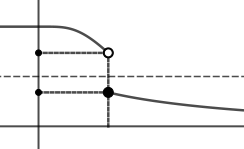
\includegraphics[width=5.5cm]{Images/lemma}};
				\draw [color=black](0.75,-0.05) node[anchor=north west] {$\alpha(c)$};
				\draw [color=black](1.95,0.4) node[anchor=north west] {$\alpha$};
				\draw [color=black](-2.2,-1.1) node[anchor=north west] {$0$};
				\draw [color=black](-0.5,-1.15) node[anchor=north west] {$c_0$};
				\draw [color=black](-2.2,1.55) node[anchor=north west] {$1$};
				\draw [color=black](-3.05,0.8) node[anchor=north west] {$\alpha(c_0-)$};
				\draw [color=black](-2.8,-0.2) node[anchor=north west] {$\alpha(c_0)$};
				\end{tikzpicture}
			\end{center}
			Pro $c_0$ takové, že $\alpha(c_0-)\geq \alpha\geq \alpha(c_0)$, definujeme  
			$$ \Phiast(\textbf{x}):=\begin{cases}
			1&f_1>c_0f_0,\\\gamma=\frac{\alpha-\alpha(c_0)}{\alpha(c_0-)-\alpha(c_0)}&f_1=c_0f_0,\\0&f_1<c_0f_0,
			\end{cases} $$ kde $\alpha(c_0-)$ značí $\lim\limits_{c\to c_0-}\alpha(c)$.
			V případě, že $\alpha(c)$ je spojitá v~$c_0$, pak číslo $\gamma$ je nedefinováno ($\frac{0}{0}$). To však nevadí, protože v~tomto případě platí
			$$ 0= \alpha(c_0-)-\alpha(c_0)=1-\alpha(c_0)-\br{1-\alpha(c_0-)}=\underbrace{\PP_{\t_0}\Br{\frac{f_1}{f_0}\leq c_0}}_{F_Y(c_0)}-\underbrace{\PP_{\t_0}\Br{\frac{f_1}{f_0}< c_0}}_{F_Y(c_0-)}=\PP_{\t_0}\Br{\frac{f_1}{f_0}=c_0}, $$ a~tedy vidíme, že množina $\{ f_1=c_0f_0\}$ má nulovou pravděpodobnostní míru. To znamená, že test $\Phiast$ je definován jednoznačně $s.j.~\PP_{\t_0}$. Hladina tohoto testu $\Phiast$ je
			\[
			\begin{split}
			\beta_{\Phiast}(\t_0)&=\E_{\t_0}\crossedphi(\X)=1\cdot \PP(\Phiast=1)+\gamma\PP(\Phiast=\gamma)+0\cdot\PP(\Phiast=0)=\\&=\underbrace{\PP(f_1>c_0f_0)}_{\alpha(c_0)}+\frac{\alpha-\alpha(c_0)}{\alpha(c_0-)-\alpha(c_0)}\cdot\underbrace{\PP(f_1=c_0f_0)}_{\alpha(c_0-)-\alpha(c_0)}=\alpha.
			\end{split}
			\]
			\item Nyní ukážeme, že zkonstruovaný test $\Phiast$ je UMP testem. Nechť $\Phiast$ je test z~předchozí části důkazu a~$\crossedphi$ je libovolný jiný test na~hladině významnosti $\alpha$, tzn. $\beta_{\crossedphi}(\t_0)\leq \alpha$. Chceme ukázat, že $\beta_{\Phiast}(\t_1)-\beta_{\crossedphi}(\t_1)\geq0$.
			\[
			\begin{split}
			&\beta_{\Phiast}(\t_1)-\beta_{\crossedphi}(\t_1)=\E_{\t_1}[\Phiast(\X)-\crossedphi(\X)]=\int\limits_{\R^n}(\Phiast-\crossedphi)f_1(\textbf{x})\d\textbf{x}=\\
			&=\underbrace{\int\limits_{S^+:=\{ \Phiast-\crossedphi>0 \}}(\Phiast-\crossedphi)f_1\d\textbf{x}}_{\textbf{x}\in S^+\Rightarrow~\Phiast>0~\Rightarrow~f_1\geq c_0f_0}+\underbrace{\int\limits_{S^-:=\{ \Phiast-\crossedphi<0 \}}(\Phiast-\crossedphi)f_1\d\textbf{x}}_{\textbf{x}\in S^-\Rightarrow~\Phiast<1~\Rightarrow~ f_1\leq c_0f_0}+\underbrace{\int\limits_{\{ \Phiast-\crossedphi=0 \}}(\Phiast-\crossedphi)f_1\d\textbf{x}}_{=0}\geq\\
			&\geq
			\int\limits_{S^+}(\Phiast-\crossedphi)c_0f_0\d\textbf{x}+ \int\limits_{S^-}(\Phiast-\crossedphi)c_0f_0\d\textbf{x}=c_0\underbrace{\int\limits_{\R^n}(\Phiast-\crossedphi)f_0\d\textbf{x}}_{\E_{\t_0}(\Phiast-\crossedphi)}=c_0\br{\underbrace{\beta_{\Phiast}(\t_0)}_{=\alpha}-\underbrace{\beta_{\crossedphi}(\t_0)}_{\leq\alpha}}\geq 0. 
			\end{split}
			\] Z~toho vyplývá, že síla testu $\Phiast$ je větší, než síla testu $\crossedphi$. Konstantu $c_0$ z~důkazu ztotožňujeme s~$K>0$ ze~znění věty.
		\end{enumerate}
	\end{proof}
\end{theorem}
\begin{dusl}\label{dusledek} Pokud platí, že $\PP_{\t_0}(f_1=Kf_0)=0$, pak můžeme psát
	$$ \Phiast=\begin{cases}
	1&x\in W^\ast=\{ f_1\geq Kf_0 \},\\0& x\in (W^\ast)^c=\{f_1<Kf_0\}.
	\end{cases} $$ Tedy v~případě, že hranice $\{f_1= Kf_0\} $ je nulové $\PP_{\t_0}$ míry, potom existuje neznáhodněný test s~UMP kritickou oblastí $W^\ast$ pro~testování $H_0$ versus $H_1$, přičemž pravděpodobnost chyby I. druhu je přímo rovna požadované signifikanci $\alpha$,  $\beta_{W^\ast}(\t_0)=\alpha$, zatímco síla testu $\beta_{W^\ast}(\t_1)$ je maximální možná.
\end{dusl}
\begin{example}
	Neyman-Pearsonovo lemma se~zpravidla používá pro~tzv. jednoduché testy, což znamená, že je testovaný parametr zadaný konkrétní jednou hodnotou. Příkladem může být třeba testování hypotéz pro~parametry $\n{\mu,\sigma^2}$ typu 
$$ \hypothesis{\mu=\mu_0}{\mu=\mu_1\neq\mu_0~(\text{resp. }\mu\gtrless\mu_0)}. $$
 Pro~složené testy, např. typu
$$ \hypothesis{\sigma^2\geq7}{\sigma^2< 7},\quad\text{nebo }\hypothesis{\mu\leq\mu_0}{\mu>\mu_0},  $$ ani jiné podobně zadané testy, optimální $\txt{UMP}_\alpha$ test nemusí obecně existovat a~jsou nutné dodatečné podmínky (viz následující sekce).
\end{example}

\section{Složené hypotézy a~MLR systémy}
\subsection*{Postup použití N-PL v~praxi pro~test z~důsledku \ref{dusledek}.}Hledáme takový test $\Phiast$ tvaru 
$$ \Phiast(\textbf{x})=\begin{cases}
1&\textbf{x}\in\{f_1\geq Kf_0\}=W^\ast\text{ ... UMP CR},\\0&\textbf{x}\in\{f_1<Kf_0\}=(W^\ast)^c,
\end{cases} $$
pro který je dosažena hladina testu $\beta_{\Phiast}(\t_0)=\alpha$, přičemž síla (silofunkce) testu $\beta$ je optimální.
\begin{enumerate}[1)]
	\item Nejdříve najdeme \textbf{tvar} $W^\ast$ jako řešení nerovnice $f_1\geq Kf_0$. Získáme ho v~nějakém tvaru $W^\ast=\{ T(\textbf{x})\geq K' \}$, resp. $W^\ast=\{ T(\textbf{x})\leq K' \}$, s~blíže nespecifikovanou volnou konstantou $K'$, tedy 
	$$\{f_1\geq Kf_0\}\sim\{T(\X)\geq K' \},$$ resp.$$\{f_1\geq Kf_0\}\sim\{T(\X)\leq K' \},$$
	kde $T(\X)$ se~nazývá \textbf{testovací statistika}.
	\item Konkrétní hodnotu $K'$ pak určíme z~rovnice  $\PP_{\t_0}\br{T(\X)\geq K'}=\alpha$, resp.  $\PP_{\t_0}\br{T(\X)\leq K'}=\alpha$. K~vyřešení této nerovnosti však nutně potřebujeme umět vyjádřit $\PP_{\t_0}(T\geq K')$, resp. \mbox{$\PP_{\t_0}(T\leq K')$} za~předpokladu platnosti hypotézy $H_0$, tzn. při~$\t_0$. Odvození rozdělení $T(\X)$ při~$\t_0$ se~říká "distributional problem"~testování hypotéz a~jde o~stěžejní část úspěšné aplikace.
	\item V~případě, že $H_1$ je složená, tzn. $H_1:\t\in\Theta_1$, postupujeme takto:
	volíme $\t_1\in\Theta_1$ libovolně pevně a~testujeme hypotézu
	$ \hypothesis{\t=\t_0}{\t=\t_1\text{ na~hladině }\alpha.} $
	Z Neyman-Pearsonova lemmatu existuje $\txt{UMP}_\alpha$ test $\Phiast$, případně UMPCR $W^\ast$. Pokud tento $\Phiast$, případně $W^\ast$, nezávisí na~volbě $\t_1$, máme finální $\txt{UMP}_\alpha$ test při~složené alternativě $H_1$.
	\item  Pokud i~$H_0$ je složená, tzn. $H_0:\t\in\Theta_0$, pak, pokud to lze, ještě navíc ukážeme, že  $\sup\limits_{\t\in\Theta_0}\beta_{\Phiast}(\t)\leq\alpha$, tzn., že $\forall\t_0'\in\Theta$, platí, že $\beta_{\Phiast}(\t_0')\leq\alpha$. Průchodnost bodů 3) a~4) zajišťuje například následující koncept MLR.
\end{enumerate}

\begin{define}
	Systém hustot $\mathcal{F}$ se~nazývá  \textbf{MLR} (\textit{Monotone likelihood ratio}), pokud \newline $\exists T(\textbf{x}):\R^n\to\R^1$ tak, že pro~$\forall\t_0<\t_1$ platí, že $\frac{f_1}{f_0}$ je monotonní funkcí statistiky $T(\textbf{x})$, tzn. \mbox{$\frac{f_1}{f_0}=g\br{T(\textbf{x})}$}, kde $g$ je monotonní. Podíl $\frac{f_1}{f_0}=\frac{L(\t_1)}{L(\t_0)}$ se~nazývá \textbf{věrohodnostním poměrem} (\textit{likelihood ratio}), ozn. $\mathrm{LR}(\textbf{x}),~\textbf{x}\in\mathcal{X}$.
\end{define}
\begin{remark}
	Pokládáme $\frac{f_1}{f_0}=+\infty$, pokud $f_1>0,~f_0=0$. Pro~$f_1=0$ a~$f_0=0$ výraz nedefinujeme. Monotonii vyžadujeme pouze tam, kde je výraz $\mathrm{LR}(\textbf{x})$ definován.
\end{remark}
\begin{theorem}\label{vetaUMP} Mějme rostoucí MLR systém hustot $\mathcal{F}$ se~statistikou $T(\X)$. Testujeme hypotézu \\
	\mbox{$ \hypothesis{\t\leq\t_0}{\t>\t_0}$}, $\t\in\R^1 $, tzv. jednostrannou hypotézu oproti~jednostranné alternativě, na~zadané hladině $\alpha\in(0,1)$.
	Pak existuje $\txt{UMP}_\alpha$ test $\Phiast$ ve~tvaru $$ \Phiast(\textbf{x})=\begin{cases}
	1 & T(\textbf{x})>K, \\ \gamma &T(\textbf{x})=K, \\ 0&T(\textbf{x})<K,
	\end{cases} $$ přičemž $K$ a~$\gamma$ jsou určeny podmínkou $\beta_{\Phiast}(\t_0)=\alpha$, tzn.  $\E_{\t_0}[\Phiast(\X)]=\alpha$, tedy $$\PP_{\t_0}\br{T(\X)>K}+\gamma \PP_{\t_0}\br{T(\X)=K}+0\cdot \PP_{\t_0}\br{T(\X)<K}	=\alpha.$$
	Pro případ klesajícího MLR systému $\mathcal{F}$ stačí v~tvrzení zaměnit nerovnosti za~opačné.
	\begin{proof} Důkaz provedeme speciálně pro~ostře rostoucí MLR systém $\mathcal{F}$.
		\begin{enumerate}[a)]
			\item Nejprve testujeme $\hypothesis{\t=\t_0}{\t>\t_0}$. Pro~tento účel zvolíme libovolně pevně $\t_1>\t_0$ a~testujeme $\hypothesis{\t=\t_0}{\t=\t_1}$.  Tím splníme překpoklady Neyman-Pearsonova lemmatu, podle něhož pak existuje UMP test $$ \Phiast(\textbf{x})=\begin{cases}
			1&f_1>K'f_0, \\ \gamma&f_1=K'f_0, \\ 0&f_1<K'f_0,
			\end{cases}  $$ tak, že $\beta_{\Phiast}(\t_0)=\alpha$. Nechť $\frac{f_1}{f_0}=g\br{T(\textbf{x})}$, kde $g$ je ostře rostoucí funkcí. Nyní upravíme podmínky do~tvaru
			$$ \left\{ \begin{array}{c}
			f_1>K'f_0	\\ f_1=K'f_0  \\ f_1<K'f_0
			\end{array}  \right\}\sim\left\{ \begin{array}{c}
			f_1/f_0>K'	\\ f_1/f_0=K'  \\ f_1/f_0<K'
			\end{array}  \right\}\sim\left\{ \begin{array}{c}
			T(\textbf{x})>\inv{g}(K')	\\ T(\textbf{x})=\inv{g}(K')  \\ T(\textbf{x})<\inv{g}(K')
			\end{array}  \right\}\sim\left\{ \begin{array}{c}
			T(\textbf{x})>K	\\ T(\textbf{x})=K  \\ T(\textbf{x})<K	\end{array}  \right\}, $$ kde  $K:=\inv{g}(K')$. Tvar testu $\Phiast$ je stejný nezávisle na~volbě $\t_1>\t_0$. Konstanty $K$ a~$\gamma$ jsou pak určeny z~rovnice $\beta_{\Phiast}(\t_0)=\alpha$, a~proto také nezávisí na~volbě $\t_1>\t_0$.		
			\item Vezmeme právě zkonstruované $\Phiast$ a~ukážeme, že pro~$\forall\t_0'<\t_0$ platí, že $\beta_{\Phiast}(\t_0')\leq \alpha$. Definujeme pomocný (čárkovaný) test $$H_0':\t=\t_0'~\text{vs.}~H_1':\t=\t_0.$$ Příslušný UMP test $H_0'$ z~N-PL má stejný tvar jako UMP $\Phiast$ zkonstruovaný v~předchozím bodě, ale na~hladině $\beta_{\Phiast}(\t_0')=\alpha'$. Jeho síla je pak rovna $\beta_{\Phiast}(\t_0)=\beta'$. 
			\item Ukážeme, že pro~UMP test $\Phiast$ platí $\alpha'\leq\beta'$. Volme test $\crossedphi(\textbf{x})=\alpha'$ pro~$\forall\textbf{x}\in\mathcal{X}$. Pak $\crossedphi$ je test $H_0'$ vs. $H_1'$ na~hladině $\alpha'$ se~silou $\alpha'$, která nemůže překročit sílu $\beta'$ UMP testu $\Phiast$, tzn. $\alpha'\leq \beta'$.
		\end{enumerate}
	\end{proof}
\end{theorem}
	\begin{example}\label{prikladek}
	Testujeme hypotézu  $H_0: \t\leq\t_0~\text{vs.}~H_1:\t>\t_0$ pro~exponenciální třídu hustot $$\mathcal{F}=\big\{ f(x,\t)=c(\t)h(x)\e{Q(\t)T(x)}:\t\in\Theta\subset\R^1 \big\}.$$ Pokud $Q(\t)$ je ryze rostoucí, resp. ryze klesající, pak $\mathcal{F}_n\equal{iid}\left\{ f(\textbf{x},\t)=\prod\limits_{i=1}^n f(x_i,\t) \right\}$ je MLR systém hustot se~statistikou $T(\textbf{x})=\sum\limits_{i=1}^n T(x_i)$. Z~věty \ref{vetaUMP} pak plyne konkrétní tvar $\txt{UMP}_\alpha$ testu $\Phiast$ pro~testování $H_0$ vs. $H_1$.
Díky této MLR exponenciální třídě hustot umíme najít stejnoměrně optimální UMP testy například pro~následující parametry specifických rozdělení:
\[
\begin{split}
H_0:p\leq p_0~\text{vs.}~H_1:p>p_0,&\quad\text{v~případě }X\sim\mathrm{Bi}(n,p),\\
H_0:\lambda\leq\lambda_0~\text{vs.}~H_1:\lambda>\lambda_0,&\quad\text{v~případě } X\sim\mathrm{Po}(\lambda),\\
\hypothesis{\t\leq\t_0}{\t>\t_0},&\quad\text{pro případ }X\sim\mathrm{Exp}(\t),\\
\hypothesis{\mu\leq\mu_0}{\mu>\mu_0},&\quad\text{při modelu }X\sim\NN(\mu,\sigma^2\text{ známé}),\text{ atp.}
\end{split}
\]
\end{example}
\section{Nestranné UMP testy (UMPU)}
V aplikacích TSH v~praxi vyvstává nutnost testovat další složitější hypotézy, jako například \[
	\begin{split}
	H_0:&~\t=\t_0~\text{vs.}~H_1:\t\neq\t_0,\quad\text{nebo} \\
	H_0:&~\t_1\leq \t\leq\t_2~\text{vs.}~H_1:\t\notin[\t_1,\t_2].
	\end{split}
	\]
	Pro takovéto případy, kdy alternativní hypotéza $H_1$ je tzv. oboustranná ($\t<\t_1$ nebo $\t>\t_2$), zpravidla neexistuje stejnoměrně nejsilnější $\txt{UMP}\alpha$ test $\Phiast$ na~hladině $\alpha$ a~jsme nuceni z~optimality UMP testu slevit. Zavedeme proto UMPU testy.
	
\begin{define}	
	Testujme $H_0:\t\in\Theta_0~\text{vs.}~H_1:\t\in\Theta_1$.
	Test $\crossedphi$ se~nazývá nestranný, pokud $\sup\limits_{\t\in\Theta_0}\beta_\crossedphi(\t)\leq \inf\limits_{\t\in\Theta_1}\beta_\crossedphi(\t)$.
\end{define}
\begin{theorem}\label{zobecneni}
	Každý UMP test $\Phiast$ je nestranný, tzn. $\silofunkceast{0}\leq\silofunkceast{1}$, tj. $$\sup\limits_{\t\in\Theta_0}\beta_{\Phiast}(\t)\leq\inf\limits_{\t\in\Theta_1}\beta_{\Phiast}(\t).$$
	\begin{proof}
		Volme $\crossedphi(\textbf{x})=\widetilde{\alpha}=\sup\limits_{\t\in\Theta_0}\beta_{\Phiast}(\t)$ pro~$\forall\textbf{x}\in\mathcal{X}$. Pak
		\[
		\begin{split}
		\silofunkce{0}&=\E_{\t_0}\crossedphi(\X)=\widetilde{\alpha},~~~\forall\t_0\in\Theta_0,\quad\text{(hladina testu $\crossedphi$)} \\\silofunkce{1}&=\E_{\t_1}\crossedphi(\X)=\widetilde{\alpha},~~~\forall\t_1\in\Theta_1.\quad\text{(silofunkce testu $\crossedphi$)}
		\end{split}
		\] 
		Podle předpokladu je $\Phiast$ UMP, a~tedy jeho silofunkce je stejnoměrně na~$\Theta_1$ vyšší, než u~všech ostatních testů včetně testu $\crossedphi$. Proto platí, že $\beta_{\Phiast}(\t_1)\geq\widetilde{\alpha}$ pro~$\forall\t_1\in\Theta_1$. Věta \ref{zobecneni} zobecňuje výsledek z~bodu c) z~důkazu věty \ref{vetaUMP}.
	\end{proof}
\end{theorem}

\begin{define}
	Stejnoměrně nejsilnější test mezi~všemi nestrannými testy se~nazývá UMPU. (\textit{UMP Unbiased}).
\end{define}


\begin{theorem} \label{UMPU}
	Testujeme hypotézu	$H_0:\t=\t_0~\text{vs.}~H_1:\t\neq\t_0,$ kde $\t\in\Theta\subset\R^1$ a~$\t_0$ je vnitřním bodem $\Theta$, tedy , $\t_0\in\Theta^\circ$. Nechť $\mathcal{F} $ je exponenciální třída hustot z~příkladu \ref{prikladek} s~$Q(\t)$ ryze rostoucí a~diferencovatelnou, tedy $\mathcal{F}_n=\left\{ f(\textbf{x},\t)\equal{iid}\prod\limits_{i=1}^n f(x_i,\t) \right\}$ je MLR systém se~statistikou $T(\textbf{x})=\sum_{i=1}^n T(x_i)$. Pak existuje $\txt{UMPU}_\alpha$ test tvaru  $$\Phiast_u(\textbf{x})=\begin{cases}
	1&T(\textbf{x})<K_1~\vee~T(\textbf{x})>K_2,\\\gamma_1&T(\textbf{x})=K_1,\\\gamma_2&T(\textbf{x})=K_2,\\0&T(\textbf{x})\in(K_1,K_2),
	\end{cases}$$ takový, že $\beta_{\Phiast_u}(\t_0)=\alpha$. Konstanty $K_1,K_2,\gamma_1,\gamma_2$ určíme tak, aby byla splněna podmínka $$\PP\br{T(\X)<K_1}+\PP\br{T(\X)>K_2}+\gamma_1\PP\br{T(\X)=K_1}+\gamma_2\PP\br{T(\X)=K_2}=\alpha.$$
	\begin{proof}
		Bez důkazu. (ze zobecněného N-PL)
	\end{proof}
\end{theorem}
Na základě věty \ref{UMPU} umíme nalézt alespoň $\txt{UMPU}_\alpha$ optimální testy mezi~všemi nestrannými testy, např. pro~hypotézy ve~tvaru 
\[
\begin{split}
\hypothesis{\mu=\mu_0}{\mu\neq\mu_0},&\quad\text{při~Gaussovském modelu  }X\sim\NN(\mu,\sigma^2~\text{známé}),\\
\hypothesis{\sigma^2=\sigma^2_0}{\sigma^2\neq\sigma_0^2},&\quad\text{při~Gaussovském modelu } X\sim\NN(\mu\text{ známé},\sigma^2).
\end{split}
\]

\begin{example}[Podrobněji viz MASC]
	Mějme $X_1,...,X_n~iid~\n{\mu,\sigma^2}$, kde $\sigma^2$ známe. Testujme hypotézu \mbox{$\hypothesis{\mu=\mu_0}{\mu\neq\mu_0}$}.
	Za účelem nalezení $\txt{UMP}_\alpha$ volíme $\mu_1\neq\mu_0$ a~testujeme  $\hypothesis{\mu=\mu_0}{\mu=\mu_1}$. Z~N-PL určíme tvar kritické oblasti 
	$$ W^\ast=\left\{ \textbf{x}\in\R^n:f_1(\textbf{x})\geq Kf_0(\textbf{x}) \right\}=\left\{ (\mu_1-\mu_0)\sm{j=1}{n}x_j\geq K' \right\}, $$
	kde do~$K'$ byly zahrnuty všechny konstanty nezávislé na~$\textbf{x}$. Nyní, pokud $\mu_1>\mu_0$, pak $W^\ast=\left\{ \sumjn x_j\geq K'' \right\}$, je-li $\mu_1<\mu_0$, pak $W^\ast=\left\{ \sumjn x_j\leq K'' \right\}$. Protože se~tvar $W^\ast$ takto mění v~závislosti na~volbě $\mu_1\gtrless \mu_0$, nelze najít stejnoměrně univerzální kritickou oblast $W^\ast$ pro~celý obor $H_1:\mu\neq\mu_0$. Z~toho vyplývá, že $\txt{UMP}_\alpha$ test neexistuje. 
	
	Umíme však nalézt $\txt{UMPU}_\alpha$ z~věty \ref{UMPU}, protože Gaussovská rodina $\n{\mu,\sigma^2\text{ známé}}$ je z~exponenciální třídy hustot s~příslušnými $Q(\mu)=\frac{\mu}{\sigma^2}$ a~$T(\X)=\sumjn X_j$ (vzhledem k~$\mathcal{F}_n$). Rozdělení testovací statistiky $T(\X)$ za~platnosti $H_0:\mu=\mu_0$ umíme vyřešit: \\$T(\X)\big|_{H_0}\sim\n{n\mu_0,n\sigma^2}$. Volíme-li ve~větě \ref{UMPU} konstatny $K_1$ a~$K_2$ symetricky, dostáváme $\txt{UMPU}_\alpha$ CR ve tvaru \mbox{$W^\ast=\left\{ \frac{\sqrt{n}\abs{\oxn-\mu_0}}{\sigma}\geq K_1' \right\}$}. Pro tuto novou testovací statistiku $$T^\ast(\X)=\frac{\sqrt{n}(\oxn-\mu_0)}{\sigma}\sim\n{0,1}$$ můžeme snadno určit $K_1'=u_{1-\frac{\alpha}{2}}$ kvantil $\n{0,1}$ tak, že platí $$ \beta_{W^\ast}(\mu_0)=\p{\text{chyby I. druhu}}=\p{\frac{\sqrt{n}\abs{\oxn-\mu_0}}{\sigma}\geq u_{1-\frac{\alpha}{2}}}=\alpha. $$
\end{example}